\documentclass[paper=letter,11pt]{scrartcl}

\KOMAoptions{headinclude=true, footinclude=false}
\KOMAoptions{DIV=14, BCOR=5mm}
\KOMAoptions{numbers=noendperiod}
\KOMAoptions{parskip=half}
\addtokomafont{disposition}{\rmfamily}
\addtokomafont{part}{\LARGE}
\addtokomafont{descriptionlabel}{\rmfamily}
%\setkomafont{pageheadfoot}{\normalsize\sffamily}
\setkomafont{pagehead}{\normalsize\rmfamily}
%\setkomafont{publishers}{\normalsize\rmfamily}
\setkomafont{caption}{\normalfont\small}
\setcapindent{0pt}
\deffootnote[1em]{1em}{1em}{\textsuperscript{\thefootnotemark}\ }


\usepackage{amsmath}
\usepackage[varg]{txfonts}
\usepackage[T1]{fontenc}
\usepackage{graphicx}
\usepackage{xcolor}
\usepackage[american]{babel}
% hyperref is needed in many places, so include it here
\usepackage{hyperref}

\usepackage{xspace}
\usepackage{multirow}
\usepackage{float}


\usepackage{braket}
\usepackage{bbm}
\usepackage{relsize}
\usepackage{tcolorbox}

\def\ketY{\ensuremath{\ket {\Psi}}}
\def\iGeV{\ensuremath{\textrm{GeV}^{-1}}}
%\def\mp{\ensuremath{m_{\textrm{proton}}}}
\def\rp{\ensuremath{r_{\textrm{proton}}}}
\def\me{\ensuremath{m_{\textrm{electron}}}}
\def\aG{\ensuremath{\alpha_G}}
\def\rAtom{\ensuremath{r_{\textrm{atom}}}}
\def\rNucl{\ensuremath{r_{\textrm{nucleus}}}}
\def\GN{\ensuremath{\textrm{G}_\textrm{N}}}
\def\ketX{\ensuremath{\ket{\vec{x}}}}
\def\ve{\ensuremath{\vec{\epsilon}}}


\def\ABCDMatrix{\ensuremath{\begin{pmatrix} A &  B  \\ C  & D \end{pmatrix}}}
\def\xyprime{\ensuremath{\begin{pmatrix} x' \\ y' \end{pmatrix}}}
\def\xyprimeT{\ensuremath{\begin{pmatrix} x' &  y' \end{pmatrix}}}
\def\xy{\ensuremath{\begin{pmatrix} x \\ y \end{pmatrix}}}
\def\xyT{\ensuremath{\begin{pmatrix} x & y \end{pmatrix}}}

\def\IMatrix{\ensuremath{\begin{pmatrix} 0 &  1  \\ -1  & 0 \end{pmatrix}}}
\def\IBoostMatrix{\ensuremath{\begin{pmatrix} 0 &  1  \\ 1  & 0 \end{pmatrix}}}
\def\JThree{\ensuremath{\begin{pmatrix}    0 & -i & 0  \\ i & 0  & 0 \\ 0 & 0 & 0 \end{pmatrix}}} 
\def\JTwo{\ensuremath{\begin{bmatrix}    0 & 0 & -i  \\ 0 & 0  & 0 \\ i & 0 & 0 \end{bmatrix}}}
\def\JOne{\ensuremath{\begin{bmatrix}    0 & 0 & 0  \\ 0 & 0  & -i \\ 0 & i & 0 \end{bmatrix}}}
\def\etamn{\ensuremath{\eta_{\mu\nu}}}
\def\Lmn{\ensuremath{\Lambda^\mu_\nu}}
\def\dmn{\ensuremath{\delta^\mu_\nu}}
\def\wmn{\ensuremath{\omega^\mu_\nu}}
\def\be{\begin{equation*}}
\def\ee{\end{equation*}}
\def\bea{\begin{eqnarray*}}
\def\eea{\end{eqnarray*}}
\def\bi{\begin{itemize}}
\def\ei{\end{itemize}}
\def\fmn{\ensuremath{F_{\mu\nu}}}
\def\fMN{\ensuremath{F^{\mu\nu}}}
\def\bc{\begin{center}}
\def\ec{\end{center}}
\def\nus{$\nu$s}

\def\adagger{\ensuremath{a_{p\sigma}^\dagger}}
\def\lineacross{\noindent\rule{\textwidth}{1pt}}

\newcommand{\multiline}[1] {
\begin{tabular} {|l}
#1
\end{tabular}
}

\newcommand{\multilineNoLine}[1] {
\begin{tabular} {l}
#1
\end{tabular}
}



\newcommand{\lineTwo}[2] {
\begin{tabular} {|l}
#1 \\
#2
\end{tabular}
}

\newcommand{\rmt}[1] {
\textrm{#1}
}


%
% Units
%
\def\m{\ensuremath{\rmt{m}}}
\def\GeV{\ensuremath{\rmt{GeV}}}
\def\pt{\ensuremath{p_\rmt{T}}}


\def\parity{\ensuremath{\mathcal{P}}}

\usepackage{cancel}
\usepackage{ mathrsfs }
\def\bigL{\ensuremath{\mathscr{L}}}

\usepackage{ dsfont }



\usepackage{fancyhdr}
\fancyhf{}


\lhead{\Large 33-444} % \hfill Introduction to Particle Physics \hfill Spring 2019}
\chead{\Large Introduction to Particle Physics} % \hfill Spring 2019}
\rhead{\Large Spring 2019} % \hfill Introduction to Particle Physics \hfill Spring 2019}
\begin{document}
\thispagestyle{fancy}





%\begin{tabular}{c}
%{\large 33-444 \hfill Intro To Particle \hfill Spring 2019\\}
%\hline 
%\end{tabular}

\begin{center}
{\huge \textbf{Final}}
\large

\end{center}

{\large



\textbf{1) What are three major consequences of combining QM and Relativity?}\hfill \textit{(3 points)}\\

Many possible answers, some I had in mind...\\
- Anti-particles\\
- Connection between spin and statistics\\
- Only contain certain types of leading interactions


\vspace{0.5in}


\textbf{2) Lorentz Transforms } \hfill \textit{(4 points)}\\
\begin{itemize}
\item[a)] How does a \textbf{massive} particle $\ket{p^\mu,\sigma}$ transform under a general Lorentz transformation ($\Lambda_\mu^\nu$) ?
$\Lambda_\mu^\nu \ket{p^\mu,\sigma} = \sum_{\sigma'} R_{\sigma \sigma'} \ket{\Lambda p,\sigma'}$, where R is a rotation matrix.
\item[b)] How does a \textbf{mass-less} particle $\ket{p^\mu,\sigma}$ transform under a general Lorentz transformation ($\Lambda_\mu^\nu$)?
$\Lambda_\mu^\nu \ket{p^\mu,\sigma} = e^{ih\theta} \ket{\Lambda p,\sigma'}$, where h is the particles helicity.
\end{itemize}



\textbf{3) What are two restrictions to the interactions of mass-less particles that are a consequence gauge invariance ? }\hfill \textit{(2 points)}\\

Again there are many, here are a few that I have in mind.\\
-) Charge conservation\\
-) Principle of equivalence\\
-) Mass-less Spin-1 particles have to couple to particles of the same mass\\
-) Cannot have mass-less interacting particles with spin > 2.



\textbf{4) Why do the weak and strong interactions look so different from the electromagnetic interaction despite the fact that at short distances they are all described by similar Feynman diagrams with similar coupling constants?} \hfill \textit{(2 points)}\\

\bc
Weak force has massive force carriers.\\
Strong force has a coupling the gets stronger at large distances
\ec


\clearpage

\textbf{5) Muon decays: } \hfill \textit{(8 points)}\\
\begin{itemize}
  \item[a)]{ The muon decays via the weak interaction.  At low energy ($E << m_W$), this can be approximated as a point-like interaction. 
  Draw the diagram describing muon decay to an electron assuming a point-like weak interaction. 
\bc
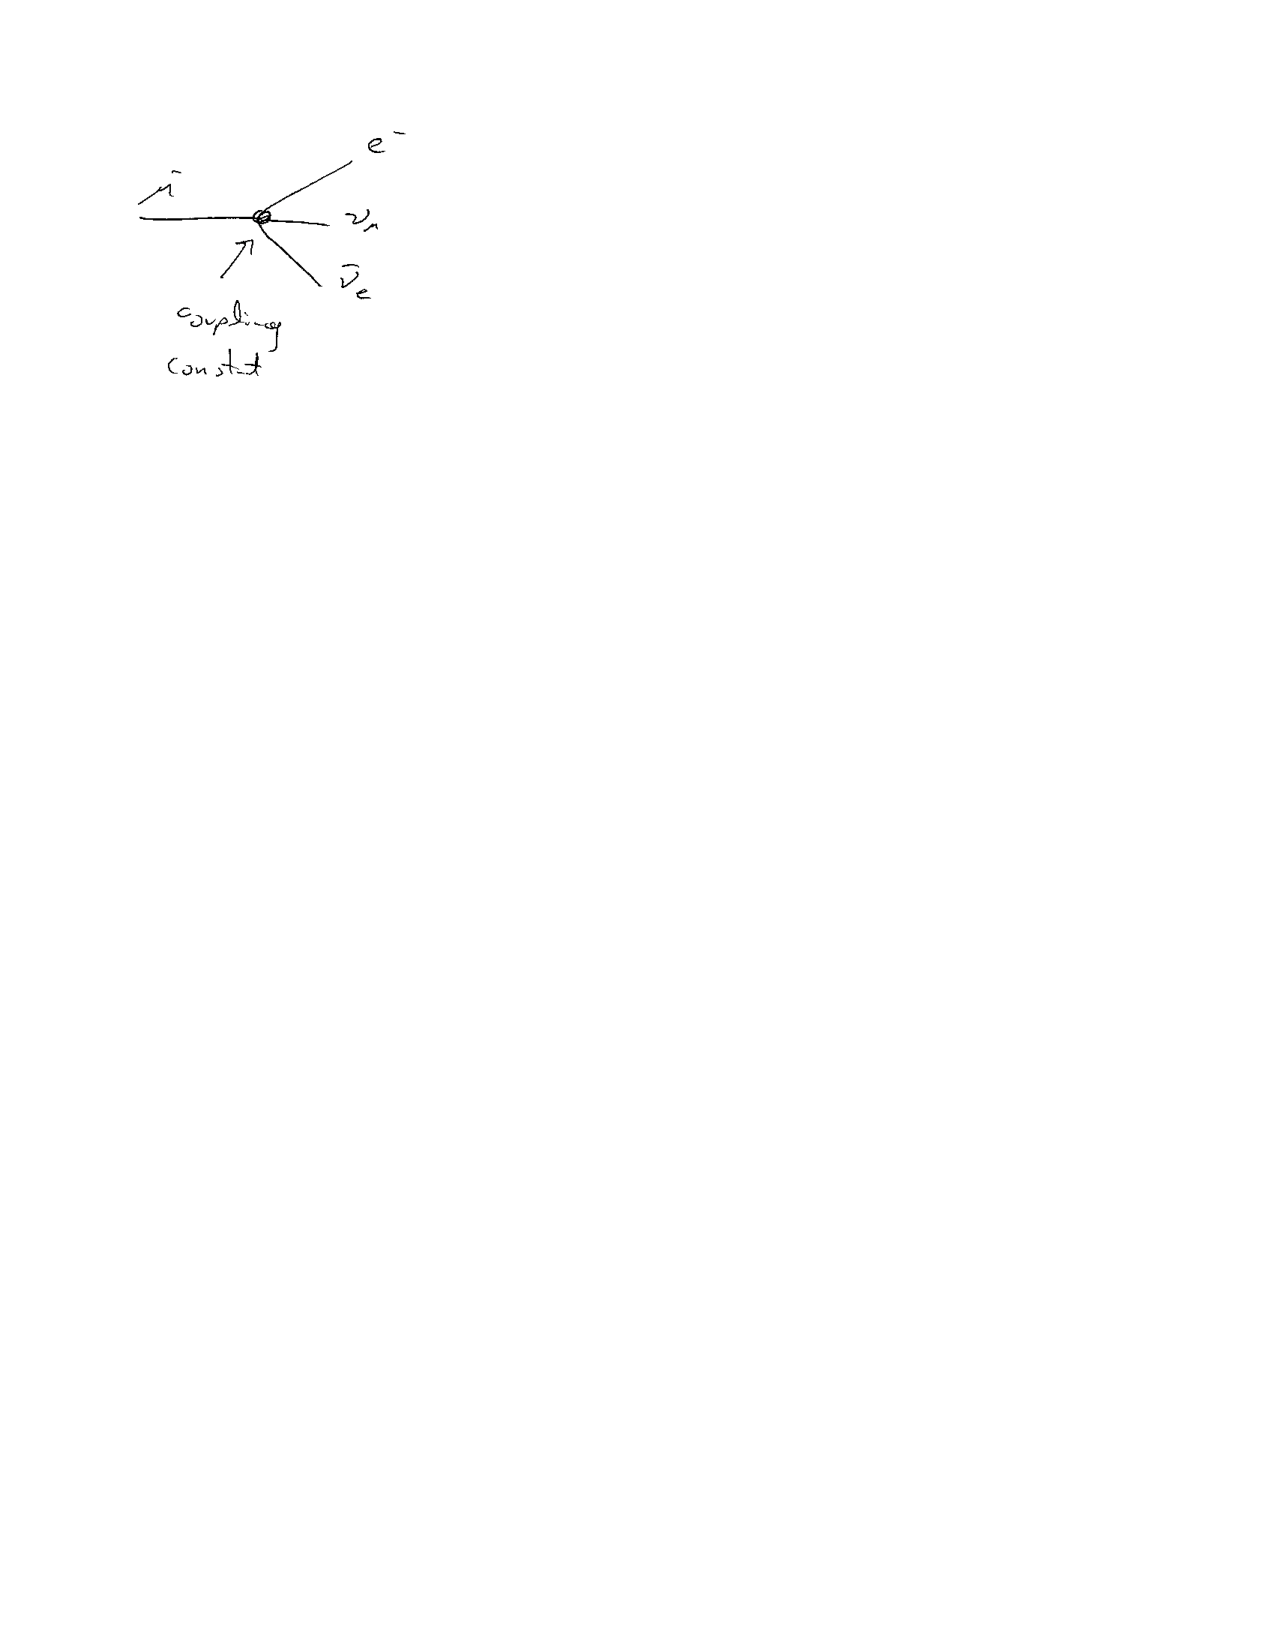
\includegraphics[width=0.3\textwidth]{./4pointInteraction.pdf}
\ec

}
  \item[b)]{What are the dimensions of the coupling constant, associated to this diagram  ?

\be
4 \times \frac{3}{2} + \rmt{[coupling constant]} = 4
\ee

$\Rightarrow$
\be
 \rmt{[coupling constant]} \sim  -2\ \rmt{or}\ \GeV^{-2}
\ee

  }
  \item[c)]{ How does the decay rate $\Gamma$ (decays/unit time)  depend on the muon mass ? 
\be
\Gamma \sim |M|^2 \sim  \rmt{[coupling constant]}^2 = \GeV^{-4}
\ee

But we also know that $\Gamma$ has to come out to have overall dimensions of $\frac{1}{\rmt{time}}$ or \GeV.

$\Rightarrow$  
\be
\Gamma \sim m_\mu^5
\ee
}
  \item[d)]{ The muon has a mass of $\sim$0.1 GeV and a lifetime of $\sim 1 \mu s$. The tau lepton has a mass of {$\sim$1 GeV}. Estimate the lifetime of the tau lepton in $\mu s$.
$m_\mu \sim 0.1 \GeV$, $m_\tau \sim 1 \GeV$, $\tau_\mu \sim 1\mu s$

Now from c) 
\be
\Gamma_\tau \sim m_\tau^5
\ee

and we know
\bea
\tau_\mu = \Gamma_\mu^{-1}\\
\tau_\tau = \Gamma_\tau^{-1}
\eea

so, 

\be
\frac{\tau_\tau}{\tau_\mu} = \frac{\Gamma_\mu}{\Gamma_\tau}
\ee

$\Rightarrow$
\be
\tau_\tau = \tau_\mu \frac{\Gamma_\mu}{\Gamma_\tau} = \tau_\mu \frac{m_\mu^5}{m_\tau^5} = \tau_\mu \left(\frac{m_\mu}{m_\tau}\right)^5  = 1\mu s (10^{-1})^5 = 10^{-6} s \times 10^{-5} = 10^{-11} s
\ee


}
\end{itemize}


\textbf{6) Electron-positron Collisions } \hfill \textit{(8 points)}\\
\begin{itemize}
\item[a)]{Consider electron-positron collisions with a center-of-mass  energy of 40 GeV.
Estimate the ratio of jet production to di-muon production. 

The allowed ``jets'' are  uu, cc (with charge +2/3), and dd, ss, bb with charge (-1/3) all have a factor of 3 for color\\

\be
\frac{\sigma(ee\rightarrow jets)}{\sigma(ee\rightarrow\mu\mu)} = 3\times \sum Q^2 = 3 \times \left( (\frac{2}{3})^2 + (\frac{2}{3})^2+ (\frac{-1}{3})^2  + (\frac{-1}{3})^2 + (\frac{-1}{3})^2  \right) = 3 \times \frac{11}{9} = \frac{11}{3}
\ee

}
\item[b)]{Sketch a graph of the total cross section of $ee\rightarrow\mu\mu$ as a function of $E_{CM}$ from 40 GeV to 200. 
Also sketch the component of the cross section due to the electro-magnetic interaction.

\bc
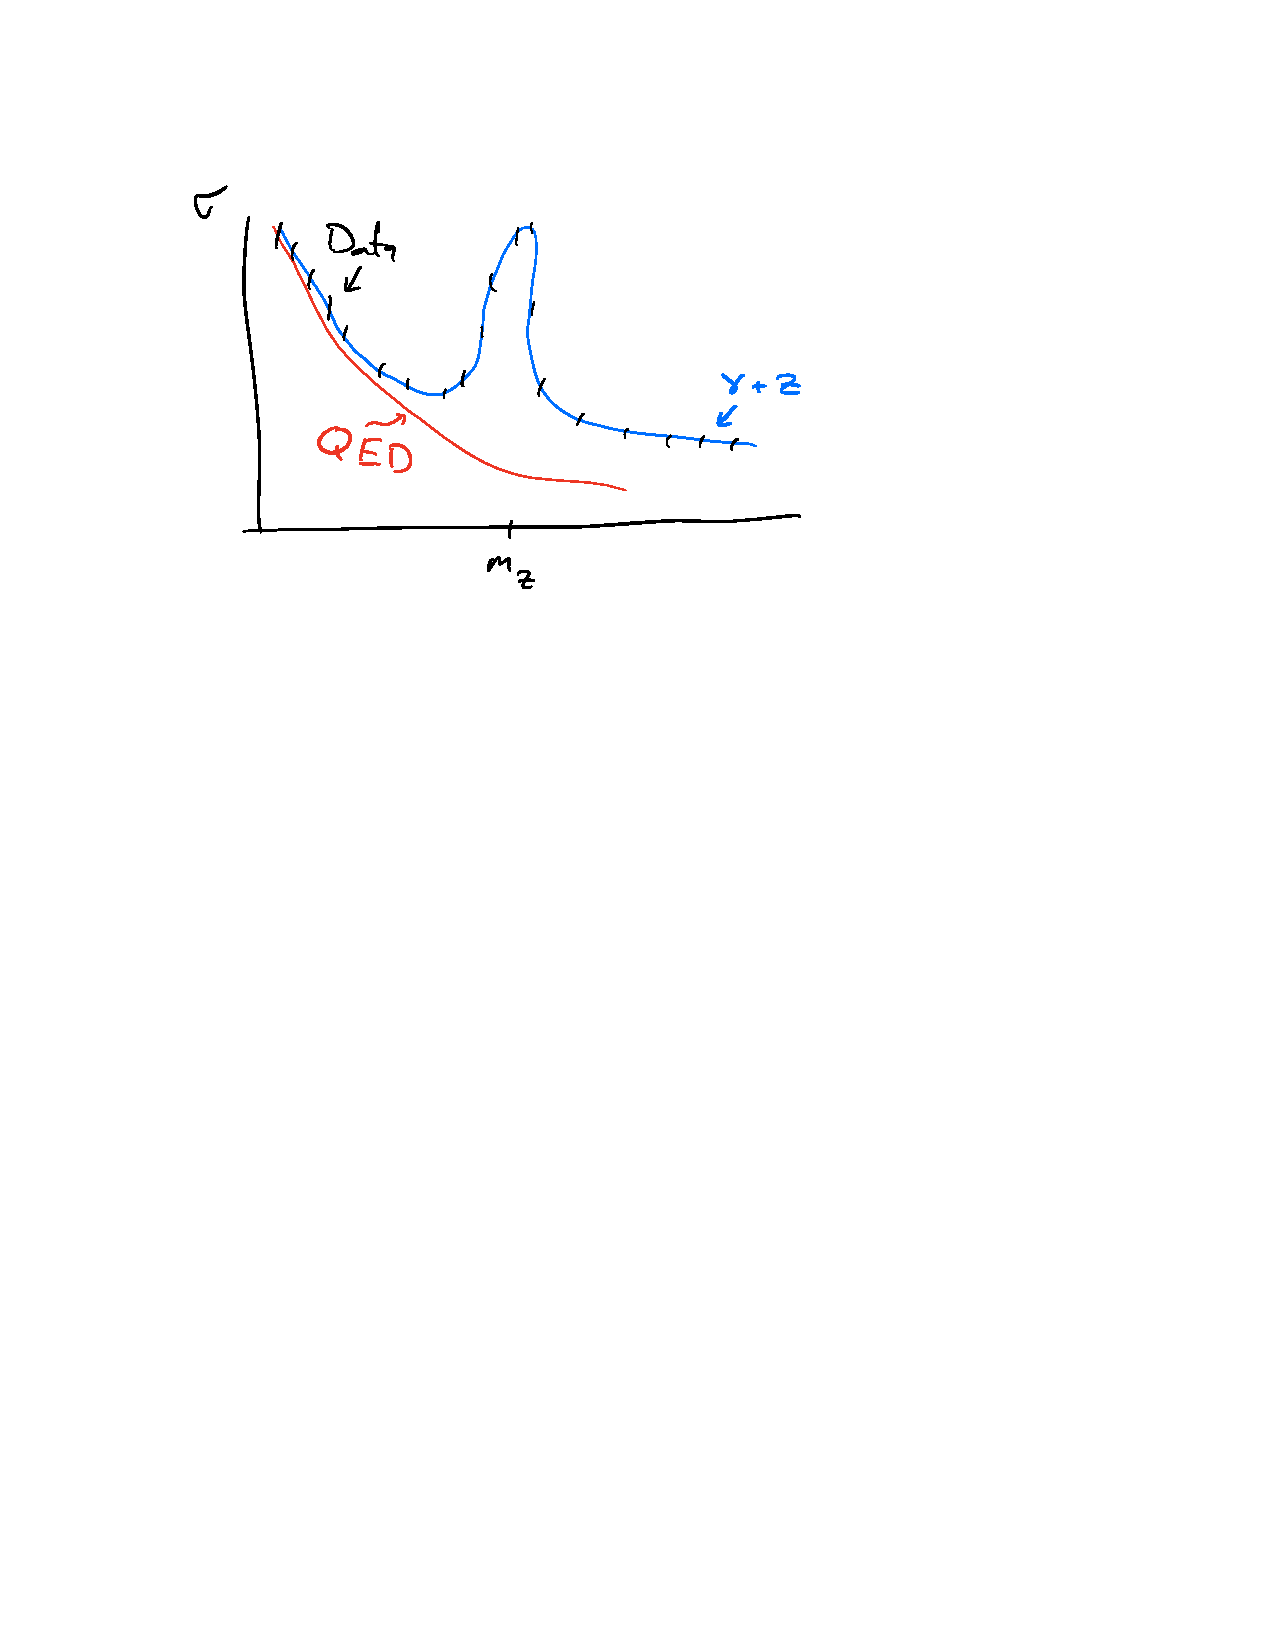
\includegraphics[width=0.4\textwidth]{./ZPeak.pdf}
\ec


}
\end{itemize}

\clearpage

\textbf{7) Branching ratios:  } \hfill \textit{(6 points)}\\
\begin{itemize}
\item[a)]{How often does a $\tau$ decay to a charged lepton ? \\ \textit{(HINT: you can neglect $\tau$ decays to charm and strange quarks) }  

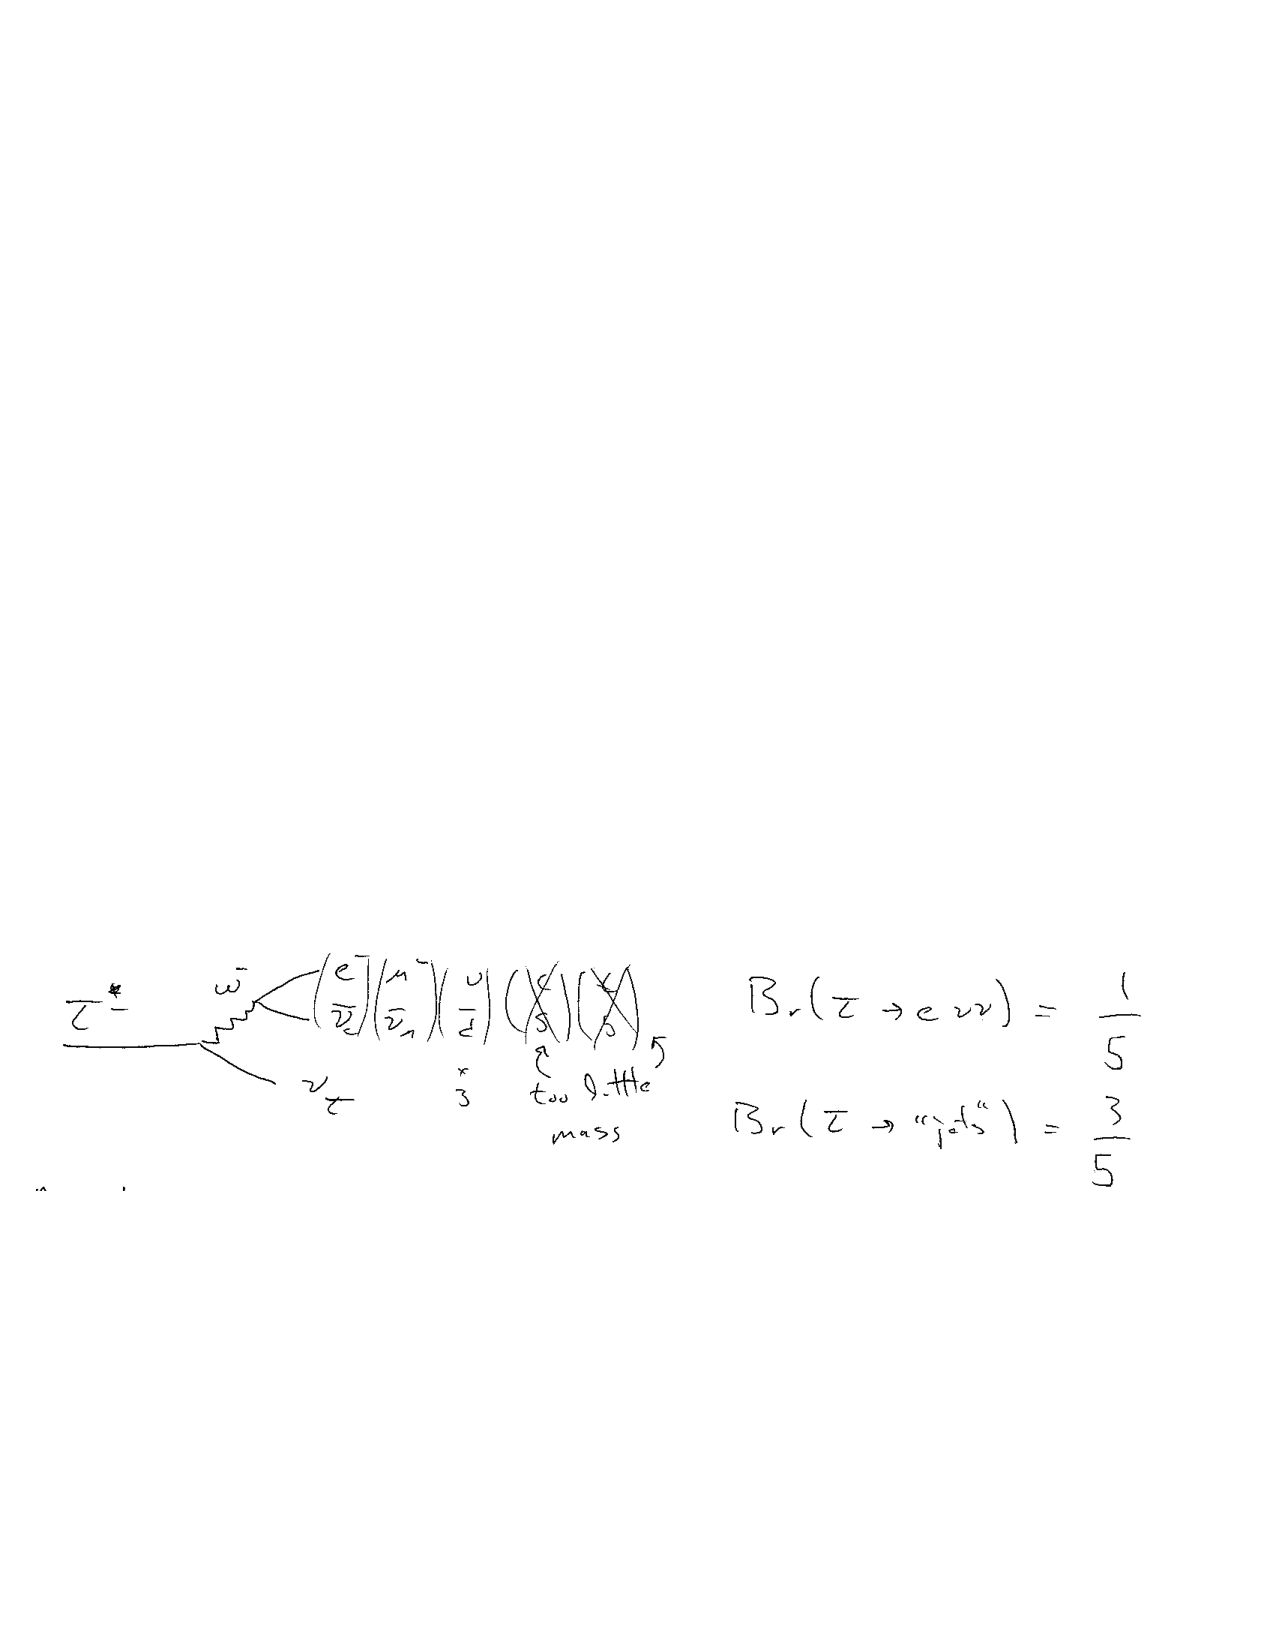
\includegraphics[width=1.0\textwidth]{./tauDecays.pdf}

So a charged lepton is $\frac{2}{5}$

}
\item[b)]{How often does a $Z$-boson decay to charged leptons ?

\bea
Br(Z\rightarrow ee)  &=&  \frac{\Gamma(Z\rightarrow ee)}{\sum_f \Gamma(Z\rightarrow ff)}  \underbrace{=}_{\rmt{Assume Universal Coupling}} \frac{  |M_0|^2}{   \sum_f |M_0|^2}  = \frac{1}{21}\\
&=& \underbrace{\frac{1}{6 + 3 \times 5}}_{\multiline{$6 = \{e,\mu,\tau,3\nu\} + $ \\ 3 colors $\times$ 5 light quarks}}
\eea

So any charged lepton is $\frac{3}{21}$

}
\item[c)]{How often does a $W$-boson decay to a charged lepton ?

\be
Br(W\rightarrow \ell \nu)  = \frac{1}{\underbrace{3}_{\rmt{leptons}} + \underbrace{3}_{\rmt{color}} \times \underbrace{2}_{\rmt{2 quark generations}}} = \frac{1}{9} = 0.11
\ee

So any charged lepton is $\frac{3}{9}$.

}
\end{itemize}


\textbf{8) If you want to improve momentum resolution, is it better to have a tracking detector that is twice as big or that has twice the magnetic field ?  Justify your answer.} \hfill \textit{(3 points)}\\

\be
F = ma \Rightarrow m v^2/r_c = qvB  \Rightarrow r_c = p_T/qB
\ee
Now,
\be
r_c^2 = \left(\frac{L}{2}\right)^2 + (r_c -s )^2
\ee
Or (Ignoring terms 
\be
\frac{L^2}{4} = 2 r_c s - s^2
\ee
B/c $r_c >> s$, can safely drop $s^2$ relative to $r_c s$.  Thus
\be
s = \frac{L^2}{8r_c} = \frac{qBL^2}{8p_T}
\ee

L more important than B.


\textbf{9) Spontaneous Symmetry Breaking  } \hfill \textit{(6 points)}\\
\begin{itemize}
\item[a)]{ What is the particle spectra (ie: for each particle, is it massive or mass-less and what is the spin) from the Lagrangian: \be\mathcal{L} = (\partial_\mu \phi^*) (\partial^\mu \phi) - V(\phi), \textrm{ where } \phi = \phi_1 + i \phi_2,\  V(\phi) = \mu^2\phi^*\phi + \lambda (\phi^*\phi)^2\textrm { and } \lambda, \mu^2 > 0   \ee

\bc
Two scalars, both massive.
\ec

}
\item[b)]{ What is the particle spectra from the setup in a) but with $\mu^2 < 0$ ?

\bc
Two scalars, one massive, one mass-less.  
\ec

}
\end{itemize}


\textbf{10) What is experimental evidence against a fourth generation of leptons ? } \hfill \textit{(4 points)}\\
Other than the fact that they have not be directly observed.

\bc
Measured width of the Z is sensitive to invisible neutrino decays.
\ec

\textbf{11) Neutrino Physics } \hfill \textit{(10 points)}\\
\begin{itemize}
\item[a)]{How was the distinction between \numu\ and \nue\ discovered ?

Neutrino beams, or a $\nu$ hitting something and spitting out a $\mu$.

}

\item[b)]{Why was the distinction between \numu\ and \nue\  expected ?

If only one $\nu$ then large $Br(\mu \rightarrow e \gamma)$

}
\item[c)]{What was the main reason to study \nus\ in the 60s and 70s, before we knew they had mass?

To study the weak interaction, $\nu$s only feel the weak interaction. Other particles swamped by EM or strong force.

}
\item[d)]{What are dominant kind(s) (indicate particle or anti-particle and flavor) of \nus\ that are produced (ignore oscillations) from:
\begin{itemize}
\item[i)]{ The sun ? 

$\nu_e$

} 
\item[ii)]{Nuclear reactors ? 

$\bar{\nu}_e$

}
\item[ii)]{Cosmic-rays ? 

both $\nu_\mu$ and $\nu_e$ 
(will get twice as many $\nu_\mu$s)

both neutrinos and anti-neutrinos

}
\item[iv)]{$\nu$-beams ?

both $\nu_\mu$ and $\nu_e$ 
(will typically get twice as many $\nu_\mu$s)

both neutrinos and anti-neutrinos

}
\end{itemize}
}
\end{itemize}


\textbf{12) In a two $\nu$ model, what combination of $\Delta m^2$, E, and L do the transition probabilities depend on?  } \hfill \textit{(3 points)}\\

\be
\frac{\Delta m^2 L}{E}
\ee

\textbf{13) What was the solar neutrino puzzle ? How was it resolved?  } \hfill \textit{(3 points)}\\

\bc
Fewer neutrinos from the sun than expected. 
Neutrino oscillations.
\ec


\textbf{14) What are the three fundamental length scales in nature and their associated problems.  } \hfill \textit{(3 points)}\\

\bc
Planck/Gravity scale: What replaces space-time at small distances?\\
Weak scale:  Why is gravity so weak ? Why are there big things in the Universe? \\
Hubble/Cosmological scale:  Why is the universe so big ? \\
\ec



} % Begning Large
\end{document}
